% Sample LaTeX file for creating a paper in the Morgan Kaufmannn two
% column, 8 1/2 by 11 inch proceedings format.

\documentclass[]{article}
\usepackage{proceed2e}

% Set the typeface to Times Roman
\usepackage{times}

% For figures
\usepackage{graphicx} % more modern
%\usepackage{epsfig} % less modern
\usepackage{subfigure} 
\usepackage{amssymb}
% For citations
% Citations
\usepackage[numbers]{natbib}
\bibliographystyle{abbrvnat}            % citation style in References section
\renewcommand{\bibsection}{}            % removes the References heading
\usepackage[colorlinks,citecolor=blue,urlcolor=blue,linkcolor=blue]{hyperref}
                                        % turns citations into hyperlinks



\usepackage{amsthm}
\usepackage{amsmath}
\usepackage{amssymb}
\usepackage{relsize}
\usepackage{graphicx}

\newcommand\independent{\protect\mathpalette{\protect\independenT}{\perp}}
\def\independenT#1#2{\mathrel{\rlap{$#1#2$}\mkern2mu{#1#2}}}
\newtheorem{definition}{Definition}
\newtheorem{lemma}{Lemma}
\newtheorem{theorem}{Theorem}
\newtheorem{corollary}{Corollary}
\newenvironment{claimproof}[1]{\par\noindent\underline{Proof:}\space#1}{\hfill $\blacksquare$}
\newcommand{\widesim}[2][1.5]{
  \mathrel{\overset{#2}{\scalebox{#1}[1]{$\sim$}}}}
% For algorithms
\usepackage{algorithm}
\usepackage{algorithmic}

% As of 2011, we use the hyperref package to produce hyperlinks in the
% resulting PDF.  If this breaks your system, please commend out the
% following usepackage line and replace \usepackage{icml2015} with
% \usepackage[nohyperref]{icml2015} above.
\usepackage{hyperref}

% Packages hyperref and algorithmic misbehave sometimes.  We can fix
% this with the following command.
%\newcommand{\theHalgorithm}{\arabic{algorithm}}
\newcommand*{\LargerCdot}{\raisebox{-0.25ex}{\scalebox{1.5}{$\cdot$}}}

\title{A Kernel Test for Three-Variable Interactions with Random Processes (UAI 2016)}

\author{} % LEAVE BLANK FOR ORIGINAL SUBMISSION.
          % UAI  reviewing is double-blind.

% The author names and affiliations should appear only in the accepted paper.
%
%\author{ {\bf Harry Q.~Bovik\thanks{Footnote for author to give an
%alternate address.}} \\
%Computer Science Dept. \\
%Cranberry University\\
%Pittsburgh, PA 15213 \\
%\And
%{\bf Coauthor}  \\
%Affiliation          \\
%Address \\
%\And
%{\bf Coauthor}   \\
%Affiliation \\
%Address    \\
%(if needed)\\
%}

\begin{document}

\maketitle

\begin{abstract} 

A wild bootstrap method is applied to the Lancaster three-variable interaction measure in order to detect factorisation of the joint distribution on three variables forming a stationary random process, for which existing permutation bootstrap methods fail. As in the \emph{i.i.d. } case, the Lancaster test is found to outperform existing tests in cases for which two independent variables individually have a weak influence on a third, but that when considered jointly the influence is strong. The main contributions of this paper are twofold: first, we show that the Lancaster statistic satisfies the conditions required to use the wild bootstrap; second, the way in which this is proved is novel and is simpler than existing methods, and further may be applied to other statistics.

%(An additional minor contribution is that it is also shown that the multiple testing correction proposed in [Lancaster] is too conservative, and a new correction is proposed that increases test power)
\end{abstract} 

\section{Introduction}
\label{introduction}
%Nonparametric testing of independence or interaction between random variables is a core staple of machine learning and statistics.

Nonparametric testing of independence or interaction between random variables is to machine learning and statistics as the peer review process is to publishing: everyone agrees that it is very important, but the ways in which we go about doing it in practice often rely on assumptions that probably don't hold in reality. 

Sticking to the more tractable and well-posed problem of the former, the authors observe that many existing methods in determining independence and interaction between variables rely on the assumption that the observed data are drawn \emph{i.i.d. }, which for many applications is unrealistic and restrictive \cite{gretton2005measuring}\cite{gretton2007kernel}\cite{gretton2005kernel}\cite{sejdinovic2013kernel}. Recent work has begun to extend statistical tests exploiting the theory of Reproducing Kernel Hilbert Spaces (RKHSs) from the \emph{i.i.d. } case to the time series case \cite{chwialkowski2014wild}\cite{chwialkowski2014kernel}. Of course, these tests also rely on rather restrictive assumptions on the mixing properties of the processes from which the observations are drawn; nonetheless they are a significant relaxation on the \emph{i.i.d. } assumption and are a step towards methods capable of handling more general forms of time-dependent data. 

The Lancaster interaction \cite{lancaster1969chi}\cite{sejdinovic2013kernel} is a signed measure that can be used to construct a test statistic capable of detecting dependence between three random variables. If the joint distribution on the three variables factorises in some way into a product of a marginal and a pairwise marginal, the Lancaster interaction is the zero measure. Given finite data, this can be used to construct a statistical test, the null hypothesis of which is that the joint distribution factorises thus. 	

In the \emph{i.i.d. } case, the null distribution of the test statistic can be estimated using a permutation bootstrap technique: this amounts to shuffling the indices of one or more of the variables and recalculating the test statistic on this bootstrapped data set. When our samples instead exhibit temporal dependence, shuffling the time indices destroys this dependence and thus doing so does not correspond to a valid resample of the test statistic. 

Provided that our data-generating process satisfies some technical conditions on the forms of temporal dependence, recent work by Leucht \cite{leucht2013dependent}, building on the work of Shao \cite{shao2010dependent}, can come to our rescue. The Wild Bootstrap is a method that correctly resamples from the null distribution of a test statistic, subject to certain conditions on both the test statistic and the processes from which the observations have been drawn.

In this paper we show that the Lancaster interaction test statistic satisfies the conditions required to apply the wild bootstrap procedure; moreover, the manner in which we prove this is significantly simpler than existing proofs in the literature of the same property for other kernel test statistics \cite{chwialkowski2014wild}\cite{chwialkowski2014kernel}. Our proof may be adapted from the Lancaster interaction to other test statistics. In the appendix, we provide an adaptation of the proof to the Hilbert Schmidt Independence Criterion (HSIC) test statistic, giving a significantly shorter and simpler proof than that given in \cite{chwialkowski2014kernel}. Our proof relies on a recently published version of the Central Limit Theorem for Hilbert space valued random variables \cite{dehling2015bootstrap} which may be substituted for more up-to-date theorems as further progress is made.

%
%\begin{itemize}
%\item Describe three variable interaction. It is particularly useful for cases in which any pairwise interaction is weak, but that the three variables interact strongly together.
%\item Test consists of two parts - calculating the test statistic, and bootstrapping the statistic to sample from the null in order to calculate the p-value threshold.
%\item When using time series, the difficult part is the bootstrapping because shuffling the indices breaks the temporal dependence structure.
%\item In [Leucht], they give a method for bootstrapping a certain class of statistics.
%\item The main contributions of this paper are the folllowing:
%\begin{itemize}
%\item To show that the Lancaster test statistic is such a statistic
%\item This is done using a new style of technique which in particular gives a significantly simpler proof that HSIC is also such a statistic (and thus simplifies the proofs used in [HSIC+time series])
%\item To show that the multiple testing corrections used in [Lancaster] are too conservative, and therefore that we can improve test power by using a more relaxed correction.
%\end{itemize}
%\end{itemize}
%
%
%This work combines the works of [HSIC + time series] and [Lancaster interaction] to give a non-parametric test for three variable interactions in which the samples are drawn from random processes.

\section{Main results}
The Lancaster interaction on the triple of variables $(X,Y,Z)$ is defined as the signed measure $\Delta_LP = \mathbb{P}_{XYZ} - \mathbb{P}_{XY}\mathbb{P}_{Z} - \mathbb{P}_{XZ}\mathbb{P}_{Y} - \mathbb{P}_{X}\mathbb{P}_{YZ} + 2\mathbb{P}_{X}\mathbb{P}_{Y}\mathbb{P}_{Z}$. It is straightforward to show that if any variable is independent of the other two (equivalently, if the joint distribution $\mathbb{P}_{XYZ}$ factorises into a product of marginals in any way), then $\Delta_LP = 0$. That is, writing $\mathcal{H}_X = \{X \independent (Y,Z)\}$ and similar for $\mathcal{H}_Y$ and $\mathcal{H}_Z$, we have that

\[\mathcal{H}_X \enspace \lor \enspace \mathcal{H}_Y \enspace \lor \enspace \mathcal{H}_Z \Rightarrow \Delta_LP=0 \]

By [Lancaster], we can consider mean embedding of this measure 
\begin{align}
 \mu_L = \int k(x,\cdot) l(y,\cdot) m(z,\cdot) \Delta_LP 
\end{align}


Given a i.i.d. sample $(X_i,Y_i,Z_i)_{i=1}^n$,  norm of the mean embedding $\mu_L$ can be empirically estimated using sample centered kernel matrices. If $a$ is a kernel and $A_{i,j} = A(X_i,x_j)$, then centered kernel matrices  $\tilde{A}$ is 
\[
\tilde{H}_{i,j} = \langle a(X_i,\cdot)-\tilde{\mu}_X, a(X_j,\cdot) -\tilde{\mu}_X \rangle,
\]
where $\tilde{\mu}_X = \frac{1}{n}\sum_{i=1}^n a(X_i,\cdot)$.  Indeed by by [Lancaster], estimator of the norm  mean embedding of the Lancaster interaction for i.i.d. samples is 
\begin{equation}\label{eqn:lancaster}
\|\hat \mu_L\|^2 = \frac{1}{n^2}\left(\tilde{K}\circ\tilde{L}\circ\tilde{M}\right)_{++}
\end{equation}
where $\circ$ is the Hadamard (element-wise) product and $A_{++} = \sum_{ij}A_{ij}$, for a matrix $A$. Latter [Lancaster] shows that, under the null hypothesis, $n \|\hat \mu_L\|^2 $ converges to some complicated distribution. By leveraging  samples i.i.d. assumption, quantiles of this difficult distribution  can be estimated using simple permutation bootstrap, and so a test procedure is proposed.

In time series setting this reasoning does not hold. It's difficult to study asymptotic disquisition of $n \|\hat \mu_L\|^2 $ for non i.i.d.  data and permutation bootstrap fails as showed in experiment \ref{wildBootstrap_is_necessary} in section [experiments]. to construct a test in this setting we will use asymptotic and bootstrap results for $\tau$-mixing. 

The null hypothesis of the Lancaster test is composed of three sub-components. In the following, we assume that $\mathcal{H}_Z$ holds; by symmetry, similar results hold for $\mathcal{H}_X$ and $\mathcal{H}_Y$.

It can be shown that the norm of the mean embedding can also be written as

\[ \|\hat \mu_L\|^2 = \frac{1}{n^2}\left(\widetilde{\tilde{K}\circ\tilde{L}}\circ\tilde{M}\right)_{++}\]

We simplify the problem to studying instead the distribution of
\[
\| \hat \mu^{(Z)}_{L,2} \|^2 =\frac{1}{n^2}\left(\overline{\overline{K}\circ\overline{L}}\circ\overline{M}\right)_{++}
\]
where e.g. 
\[
\overline{K}_{i,j} = \langle k(X_i,\cdot)-\mu_X, k(X_j,\cdot) -\mu_X \rangle,
\]
with $\mu_X$ being the population mean embedding of $X$. Precisely we prove
\begin{theorem} Suppose that $(X_i,Y_i,Z_i)_{i=1}^n$ are drawn from a process that is $\beta$-mixing with coefficients $\beta(m)$ satisfying $\sum_{m=1}^{\infty}\beta(m)^{\frac{\delta}{2+\delta}}<\infty$ for some $\delta>0$. Under $\mathcal{H}_Z$, $\lim_{n \to \infty} ( \| \hat \mu^{(Z)}_{L,2} \|^2 -\|\hat \mu_L\|^2 ) =0 $ in probability.
\end{theorem}
The statistic $\| \hat \mu^{(Z)}_{L,2} \|^2$ is much easier to study under non-i.i.d.  assumption. Indeed it can be written as a V-statics 
\[ 
V_n = \frac{1}{n^2} \mathlarger{\sum}_{1\leq i,j \leq n} \overline{\overline{k} \otimes \overline{l}}\otimes \overline{m} (S_i,S_j)
\]
where  $S_i = (X_i,Y_i,Z_i)$. The crucial observation is that
\[
 h = \overline{\overline{k} \otimes \overline{l}}\otimes \overline{m}
\]
is well behaved in the following sense 
\begin{theorem}
 $h$ is bounded symmetric Lipschitz contentious kernel, which is degenerate under $\mathcal{H}_Z$ i.e $ < Eh(S_i,\cdot),h(s,\cdot) > =0$ (  Paul i think this is easily done in RKHS using mean embedding def of Lancaster, somehow similar to what you did at the end of the proof of th 1.)
\end{theorem}
The asymptotic analysis of $V$-statistic with degenerate kernels is still difficult, but has been done in Leacht and Kacper. Additionally, Leucht showed a way to estimate quantiles of such $V$-statistic under using the  wild bootstrap. This, combined with quite simple analysis of V-stat under the alternative, in Kacper Theorem 2 \footnote{similar results present in Leucht as specific cases.}, results in statistical test see algorithm \ref{alg:Lancaster}.
\begin{algorithm}[tb]
   \caption{Test $\mathcal{H}_Z$ with Wild Bootstrap}
   \label{alg:Lancaster}
\begin{algorithmic}
   \STATE {\bfseries Input:} $\tilde{K}$, $\tilde{L}$, $\tilde{M}$, each size $n\times n$, $N$= number of bootstraps, $\alpha=$ p-value threshold
   \STATE $n\|\Delta_L\hat{P}\|^2 = \frac{1}{n}\left(\widetilde{\left( \tilde{K} \circ \tilde{L}\right) }\circ \tilde{M} \right)_{++}$
   \STATE samples = zeros(1,N)
   \FOR{$i=1$ {\bfseries to} $N$}
   \STATE Draw random matrix W according to Wild Bootstrap
   \STATE samples[$i$] = $\frac{1}{n}\left(W^\intercal\left( \widetilde{\left( \tilde{K} \circ \tilde{L}\right) }\circ \tilde{M} \right)W\right) _{++}$
   \ENDFOR
   \IF{sum($n\|\Delta_L\hat{P}\|^2 >$ samples)$>\frac{\alpha}{N}$}
   \STATE Reject $\mathcal{H}_Z$
   \ELSE
   \STATE Do not reject $\mathcal{H}_Z$
   \ENDIF
\end{algorithmic}
\end{algorithm}

The consistency results and type one error control result are provided in t he details section.




\section{Details} 

In this section we briefly introduce the theory and definitions required to understand the statement and proof of our main result. For a more in-depth introduction, see e.g. \cite{steinwart2008support}\cite{berlinet2011reproducing}\cite{scholkopf2002learning}

\subsection{Kernels and RKHS notation}

%Given an integrally strictly positive definite kernel $k$ on a set $\mathcal{X}$, the mapping induced by $k$ from $\mathcal{M(X)}$, the set of signed measures on $\mathcal{X}$, to the RKHS $\mathcal{H}_k$ of $k$ via $m \mapsto \int k(x,\cdot)dm(x)$ is injective. Given a finite sample $X_1,\ldots,X_n$ drawn from a probability distribution $\mathbb{P}_X$, the mean embedding $\mu_{\mathbb{P}_X}$ can be estimated as $\tilde\mu_{\mathbb{P}_X} = \frac{1}{n}\sum_{i=1}^{n}k(X_i,\cdot)$. 

%This idea is exploited in the construction of certain statistical tests including two sample independence testing (HSIC) - in this case, we wish to understand whether $\mathbb{P}_{XY}$ factorises as $\mathbb{P}_{X}\mathbb{P}_{Y}$ based on finite samples $(X_i,Y_i)$ drawn from $\mathbb{P}_{XY}$. We can consider distance between the empirical embeddings of the two measures via $\| \tilde\mu_{\mathbb{P}_{XY}}  - \tilde\mu_{\mathbb{P}_{X}\mathbb{P}_{Y}}\|^2$. We can then bootstrap this statistic to generate samples of it under the null hypothesis that $\mathbb{P}_{XY} = \mathbb{P}_{X}\mathbb{P}_{Y}$ to calculate a threshold distance over which we would reject the null hypothesis and conclude that the distribution does not factorise

Throughout this paper we will stick to the convention that $X,Y$ and $Z$ are random variables taking value in $\mathcal{X}, \mathcal{Y}$ and $\mathcal{Z}$, on which we define $k, l$ and $m$ respectively to be kernels. We will assume that our kernels are characteristic and bounded. We describe some notation relevant to the kernel $k$; similar notation holds for $l$ and $m$.

Associated with the kernel $k$ is a Hilbert space $\mathcal{H}_k$ of functions on $\mathcal{X}$ and a feature map $\phi_X:\mathcal{X}\longrightarrow\mathcal{H}_k$ such that $k(x,x') = \langle \phi_X(x),\phi_X(x')\rangle$. Given observations $\{X_i\}_{i=1}^n$, we write $K$ to be the \emph{Gram matrix} with entries $K_{ij} = k(X_i,X_j)$.  

We write $\mu_X := \mathbb{E}_X k(X,\cdot) \in \mathcal{H}_k$ which we call the \emph{mean embedding} \cite{smola2007hilbert} of the random variable $X$. When $k$ is \emph{characteristic} \cite{sriperumbudur2011universality}\cite{sriperumbudur2010hilbert}, the mapping from the set of probability distributions to $\mathcal{H}_k$ given by $\mathbb{P}_X \mapsto \mu_X$ is injective. When $k$ is bounded we can think of $\mu_X$ as the expectation of the $\mathcal{H}_k$-valued random variable $\phi_X(X)$. We can estimate the mean embedding with the \emph{empirical mean embedding} $\tilde{\mu}_X = \frac{1}{n}\sum_{i=1}^n k(X_i,\cdot)$ and we remark that $\tilde{k}(x,x') = \langle\phi_X(x)-\tilde{\mu}_X,\phi_X(x')-\tilde{\mu}_X\rangle$ is a kernel with feature map $\tilde{\phi}_X(X) = \phi_X(X) - \tilde{\mu}_X$. We denote by $\tilde{K}$ the Gram matrix with respect to $\tilde{k}$ and call this the \emph{empirically centred Gram matrix}. We note also that $\bar{k}(x,x') = \langle\phi_X(x)-\mu_X,\phi_X(x')-\mu_X\rangle$ is a kernel with feature map $\bar{\phi}_X(X) = \phi_X(X) - \mu_X$. We write $\bar\mu_X = \tilde\mu_X - \mu_X$, the empirical mean embedding with respect to $\bar{k}$. We denote by $\bar{K}$ the Gram matrix with respect to $\bar{k}$ and call this the \emph{population centred Gram matrix}. 

If $k$ and $l$ are kernels on $\mathcal{X}$ and $\mathcal{Y}$, then $k\otimes l$ is a kernel on $\mathcal{X}\times \mathcal{Y}$. We write $C_{XY} = \mathbb{E}_{XY}\bar{\phi}_X(X)\otimes\bar{\phi}_Y(Y)$ called the \emph{population centred covariance operator} and define $\bar{C}_{XY} = \frac{1}{n}\sum_{i=1}^n\bar{\phi}_X(X_i)\otimes\bar{\phi}_Y(Y_i)$ to be its empirical counterpart. Note that we can consider $C_{XY}$ to be an operator $\mathcal{H}_l \longrightarrow \mathcal{H}_k$, or as an element of the Hilbert space $\mathcal{H}_{k\otimes l}$. In the latter case we consider it to be the difference of the two mean embeddings $C_{XY}=\mu_{XY} - \mu_{X}\otimes\mu_{Y}$

\subsection{Hypothesis testing using the mean embedding}

The idea of injectively embedding measures into a Hilbert space can be exploited to design statistical tests of properties of one or more distributions. For example, the Maximum Mean Discrepancy (MMD) \cite{gretton2012kernel} two-sample test is motivated by the following: suppose we are given samples $\{X_i\}_{i=1}^n$ and $\{Y_j\}_{j=1}^m$ drawn \emph{i.i.d. } from distributions $\mathbb{P}$ and $\mathbb{Q}$ respectively. If our kernel is characteristic, then $\mu_\mathbb{P} = \mu_\mathbb{Q} \iff \mathbb{P} = \mathbb{Q}$. Under the assumption that $\mathbb{P} = \mathbb{Q}$, we would therefore expect the empirical embeddings $\tilde{\mu}_\mathbb{P}$ and $\tilde{\mu}_\mathbb{Q}$ to be `close' in Hilbert space norm. More precisely, we can use the squared Hilbert space norm of their difference $\|\tilde{\mu}_\mathbb{P} - \tilde{\mu}_\mathbb{Q} \|^2$ as a test statistic which, under the null hypothesis, would have distribution increasingly concentrated close to 0 as $n$ and $m$ become large \cite{gretton2012kernel}. The null distribution of this statistic can be estimated in the finite sample case by randomly relabelling the $X$s and $Y$s (in such a way that $n$ and $m$ are preserved) to arrive at asymptotically consistent p-values.

An independence test known as the Hilbert-Schmidt Independence Criterion (HSIC)\cite{gretton2007kernel}\cite{gretton2005kernel} can be constructed in a similar way: Given samples $\{(X_i,Y_i)\}_{i=1}^n$ drawn \emph{i.i.d. } from a joint distribution $\mathbb{P}_{XY}$, $X$ and $Y$ are independent if and only if $\mathbb{P}_{XY} = \mathbb{P}_X \mathbb{P}_Y \iff \mu_{\mathbb{P}_{XY}} = \mu_{\mathbb{P}_X\mathbb{P}_Y}$. Similarly to MMD, we can empirically estimate the two embeddings and use their squared Hilbert space distance  $\| \mu_{\mathbb{P}_{XY}} - \mu_{\mathbb{P}_X\mathbb{P}_Y}\|^2$ as a test statistic which, under the null hypothesis of independence, will be close to 0. The null distribution of this statistic can be estimated by randomly permuting the indices of one of the variables to estimate give asymptotically consistent p-values.

\subsection{Lancaster interaction test}

We can extend the above ideas to consider properties of distributions on three variables. The \emph{Lancaster interaction measure} \cite{lancaster1969chi}\cite{sejdinovic2013kernel} on the triple of variables $(X,Y,Z)$ is defined as the signed measure $\Delta_LP = \mathbb{P}_{XYZ} - \mathbb{P}_{XY}\mathbb{P}_{Z} - \mathbb{P}_{XZ}\mathbb{P}_{Y} - \mathbb{P}_{X}\mathbb{P}_{YZ} + 2\mathbb{P}_{X}\mathbb{P}_{Y}\mathbb{P}_{Z}$. It is straightforward to show that if any variable is independent of the other two (equivalently, if the joint distribution $\mathbb{P}_{XYZ}$ factorises into a product of marginals in any way), then $\Delta_LP = 0$. That is, writing $\mathcal{H}_X = \{X \independent (Y,Z)\}$ and similar for $\mathcal{H}_Y$ and $\mathcal{H}_Z$, we have that

\[\mathcal{H}_X \enspace \lor \enspace \mathcal{H}_Y \enspace \lor \enspace \mathcal{H}_Z \Rightarrow \Delta_LP=0 \]

Given a finite sample $(X_i,Y_i,Z_i)_{i=1}^n$, the mean embedding of the Lancaster interaction can be empirically estimated as $\Delta_L\hat{P} = \hat{\mu}_{\mathbb{P}_{XYZ}} - \hat{\mu}_{\mathbb{P}_{XY}\mathbb{P}_{Z}} - \hat{\mu}_{\mathbb{P}_{XZ}\mathbb{P}_{Y}} - \hat{\mu}_{\mathbb{P}_{X}\mathbb{P}_{YZ}} + 2\hat{\mu}_{\mathbb{P}_{X}\mathbb{P}_{Y}\mathbb{P}_{Z}}$. If any of the $\mathcal{H}_{\LargerCdot}$ hold, this norm of this quantity will concentrate on 0. We use the squared RKHS norm as a test statistic for the following:

$\mathcal{H}_0: \mathcal{H}_X \enspace \lor \enspace \mathcal{H}_Y \enspace \lor \enspace \mathcal{H}_Z $\\
$\mathcal{H}_1: \mathbb{P}_{XYZ}$ does not factorise in any way

By \cite{sejdinovic2013kernel}, we can write  

\begin{equation}\label{eqn:lancaster}
\|\Delta_L\hat{P}\|_{k\otimes l \otimes m}^2 = \frac{1}{n^2}\left(\tilde{K}\circ\tilde{L}\circ\tilde{M}\right)_{++}
\end{equation}


%Given kernels $k,l$ and $m$ on $\mathcal{X},\mathcal{Y}$ and $\mathcal{Z}$ respectively, $k\otimes l \otimes m$ defines a kernel on $\mathcal{X}\times \mathcal{Y} \times \mathcal{Z}$. We write $K, L$ and $M$ to denote the gram matrices of each kernel with respect to the observations, where for example $K_{ij} = k(X_i,X_j)$. We further write $\tilde{K}, \tilde{L}$ and $\tilde{M}$ for the empirically centred gram matrices, where for example $\tilde{K}_{ij} = k(X_i,X_j) - \frac{1}{n}\sum_ik(X_i,X_j)  - \frac{1}{n}\sum_jk(X_i,X_j) + \frac{1}{n^2}\sum_{ij}k(X_i,X_j)$. We can then write [Lancaster]



where $\circ$ is the Hadamard (element-wise) product and $A_{++} = \sum_{ij}A_{ij}$. For two gram matrices $A$ and $B$, it can be shown that $\left(A\circ\tilde{B}\right)_{++} = \left(\tilde{A}\circ\tilde{B}\right)_{++}$. Thus by considering $\tilde{K}\circ \tilde{L}$ to be the gram matrix of the kernel $\tilde{k}\otimes\tilde{l}$, we can also write

\begin{equation}\label{eqn:lancaster2}
\|\Delta_L\hat{P}\|_{k\otimes l \otimes m}^2 = \frac{1}{n^2}\left(\widetilde{(\tilde{K}\circ\tilde{L})}\circ\tilde{M}\right)_{++}
\end{equation}

We can similarly group together either of the other two pairs of Gram matrices and empirically recentre.


The next part of the statistical test is to find threshold values of the statistic beyond which we would reject the null hypothesis. Since our null hypothesis is a composite of three `sub-hypotheses', we must test each of them separately and we reject the composite null hypothesis if and only if we reject all three of the components. In the case that the observations are drawn \emph{i.i.d. }, the data can be resampled using permutation bootstrap method. For example, under $\mathcal{H}_X$, the bootstrapped dataset $\{X_{\pi(i)},Y_i,Z_i \}_{i=1}^n$ can be used to generate a valid resample of the test statistic under $\mathcal{H}_X$. 
%For more information on the details of the bootstrapping method, see \cite{sejdinovic2013kernel}.

Note that in order to achieve consistency for this test, we would need that $\mathcal{H}_0 \iff \Delta_LP = 0$. Unfortunately this does not hold - in \cite{sejdinovic2013kernel} examples are given of distributions for which $\mathcal{H}_0$ is false, and yet $\Delta_LP = 0$. At the time of writing, a characterisation of such distributions is unknown to the authors. Therefore, if we reject $\mathcal{H}_0$ then we conclude that the distribution does not factorise; if we fail to reject $\mathcal{H}_0$ then we can conclude nothing.

\subsection{Time series}
In this paper we are extending the existing Lancaster test from the \emph{i.i.d. } case to a case in which our observations are drawn from a random process. There are various formalisations of memory or 'mixing' of a random process \cite{doukhan1994mixing}\cite{bradley2005basic}\cite{dedecker2007weak}; of relevance to this paper are the following two:

\begin{definition}\cite{leucht2013dependent}
A process $(X_t)_{t}$ is \emph{$\tau$-mixing} if $\tau(r) \longrightarrow 0$ as $r\longrightarrow \infty$, where
\[\tau(r) = \sup_{l\in \mathbb{N}} \frac{1}{l} \sup_{r\leq i_1 \leq \ldots \leq i_l} \tau(\mathcal{F}_0,(X_{i_1}, \ldots, X_{i_l})) \longrightarrow 0\]
where
\[ \tau(\mathcal{M},X) = \mathbb{E} (\sup_{g \in \Lambda} | \int g(t) \mathbb{P}_{X|\mathcal{M}}(dt) -  \int g(t) \mathbb{P}_{X}(dt) |)\]
\end{definition}

\begin{definition}
A process $(X_t)_{t}$ is \emph{$\beta$-mixing} (also known as \emph{absolutely regular}) if $\beta(m) \longrightarrow 0$ as $m\longrightarrow \infty$, where
\[ \beta(m) = \frac{1}{2} \sup_n \sup \sum_{i=1}^I \sum_{j=1}^J | \mathbb{P}(A_i \cap B_j) - \mathbb{P}(A_i)\mathbb{P}(B_j)| \]
where the second supremum is taken  over all finite partitions $\{A_1,\ldots, A_I \}$ and  $\{B_1,\ldots, B_J\}$ of the sample space such that $A_i \in \mathcal{H}_1^n$ and $B_j \in \mathcal{H}_{n+m}^\infty$ and $\mathcal{H}_b^c = \sigma(X_b,X_{b+1},\ldots,X_{c})$
\end{definition}

The concept of $\beta$-mixing will be invoked when applying a central limit theorem in the next section. We will also need the following lemma:

\begin{lemma}\label{lemma:beta}
Suppose that the process $(X_t,Y_t,Z_t)_t$ is $\beta$-mixing. Then any `sub-process' is also $\beta$-mixing (for example $(X_t,Y_t)_t$ or $(X_t)_t$)
\end{lemma}

\subsection{V-statistics}
A V-statistic \cite{serfling2009approximation} of a k-argument, symmetric function $f$ given $i.i.d. $ observations $\mathcal{S}_n = \{S_1,\ldots,S_n\}$ where each $S_i \sim \mathbb{P}$ is written

\[ V(f,\mathcal{S}) =  \frac{1}{n^k} \mathlarger{\sum}_{1\leq i_1,\ldots, i_k \leq n} f(S_{i_1},\ldots,S_{i_k})\]

In this case, $V(f,\mathcal{S})$ is a biased (but asymptotically unbiased) estimator of $\mathbb{E}_{S_{i_1},\ldots S_{i_k} \sim \mathbb{P}}[f(S_{i_1},\ldots,S_{i_k})]$

In this paper we are only concerned with V-statistics for which $k=2$. We call $nV(f,\mathcal{S})$ \emph{normalised}. We call $f$ the \emph{core} of $V$ and we say that $f$ is \emph{degenerate} if, for any $s_1$, $\mathbb{E}_{S_2 \sim \mathbb{P}}[f(s_1,S_2)] = 0$, in which case we say that $V$ is a \emph{degenerate V-statistic}.

Many kernel test statistics can be viewed as normalised V-statistics which, under the null hypothesis, are degenerate. If moreover the test statistics diverge under the alternative hypothesis, the test would be consistent. Our main result is to prove that, under the null hypothesis, the Lancaster statistic is asymptotically a degenerate V-statistic.

\subsection{Wild Bootstrap}

In many frequentist statistical tests, estimates of the test statistic threshold required to achieve a given Type I error are obtained through a bootstrap resampling method. In the case of the Lancaster and HSIC tests with \emph{i.i.d. } observations, this is done by permuting the time indices of one of the variables to simulate samples from the distribution in which the permuted variable is independent of the other(s). However, this procedure relies on the \emph{i.i.d. } assumption of the data generating process - if, in fact, subsequent samples are \emph{not} independent of previous samples, then permuting the order of the time indices destroys any temporal dependence. 

If the test statistic has the form of a normalised V-statistic, then provided certain extra conditions are met, the Wild Bootstrap \cite{leucht2013dependent} is a method to directly resample the test statistic under the null hypothesis (in contrast to other methods that first generate a new simulated dataset and then compute the test statistic on this dataset). These conditions can be categorised as concerning: (1) Appropriate $\tau$-mixing of the process from which our observations are drawn; (2) The core of the V-statistic. If these conditions are met by the statistic $nV(f,\mathcal{S}_n)$, then \cite{leucht2013dependent} tell us that a random matrix $W$ can be drawn such that the bootstrapped statistic $nV_b(f,\mathcal{S}_n)=\frac{1}{n}\sum_{i,j,p,q}W_{ij}f(S_j,S_p)W_{pq}$ is distributed according to the null distribution of $nV$. The condition on $V(f,\mathcal{S})$ that is of crucial importance to this paper is that $f$ must be a degenerate core.




\subsection{Hilbert spaced random variable CLT}

In this paper we exploit a Central Limit Theorem for Hilbert space valued random variables that are functions of random processes \cite{dehling2015bootstrap}. One of the conditions required to apply this theorem concerns appropriate $\beta$-mixing of the underlying processes. This theorem is used as a black-box, and it is hoped by the authors that as further theorems concerning CLT-properties of Hilbert space random variables are developed, the conditions required of the processes may be weakened.

\section{Lancaster Interaction for Random Processes}

In this section we construct the Lancaster interaction test for random processes. The major difficulty in doing so is showing that, under the null hypothesis, the test statistic is a normalised degenerate V-statistic and therefore the Wild Bootstrap can be used to resample the test statistic and provide thresholds for desired p-values. The procedure for testing is summarised in Algorithm \ref{alg:Lancaster}.

The basic idea of the proof presented in this paper is to rewrite the test statistic as a sum of terms involving population centred gram matrices (as opposed to the empirically centred gram matrices in the presentation of the statistic in equation \ref{eqn:lancaster}). Under the null hypothesis, one of these terms is a normalised degenerate V-statistic and all of the others decay to $0$ as $n \longrightarrow \infty$. 

In contrast, existing proof methods have employed the theory of U- and V-statistics \cite{chwialkowski2014kernel,chwialkowski2014wild}; in particular, the Hoeffding decomposition of the core of a V-statistic as a sum of other cores \cite{serfling2009approximation}. This allows the rewriting of the V-statistic as a sum of other V-statistics, which under the null hypothesis decay to 0.

Both approaches amount to the same result, but they tackle the issue of centring of kernels in feature space in different ways. By appealing to a central limit theorem, the kernels are centred directly in the proof presented here. In contrast, the centring is obscured behind layers of algebra and theory in the previously presented proofs.

The approach taken in this paper can be modified to give a simpler proof that the Wild Bootstrap can be used for HSIC than that given in \cite{chwialkowski2014wild}; this proof is provided in the appendix.

The following lemma is a consequence of the Central Limit Theorem of \cite{dehling2015bootstrap}. After having written the Lancaster test statistic as a sum of terms involving population centred gram matrices, this lemma will be crucial to showing that the majority of the terms decay to 0.

\begin{lemma}\label{lemma:hilbertCLT}
Suppose that $(X_i)$ is $\beta$-mixing with coefficients $\beta(m)$ satisfying $\sum_{m=1}^{\infty}\beta(m)^{\frac{\delta}{2+\delta}}<\infty$ for some $\delta > 0$ and that $k$ is a bounded kernel on $\mathcal{X}$. Then $\|\hat\mu_X - \mu_X\|_k = O(n^{-\frac{1}{2}})$

\end{lemma}

The following Theorem gives sufficient conditions for the hypothesis of the Wild Bootstrap to be satisfied.

\begin{theorem}\label{theorem:lancasterAsymptote}
Suppose that $\mathbb{P}_{XYZ} = \mathbb{P}_{XY}\mathbb{P}_Z$ and that $(X_i,Y_i,Z_i)_{i=1}^n$ are drawn from a process that is both:

\begin{itemize}
\item $\beta$-mixing with coefficients $\beta(m)$ satisfying $\sum_{m=1}^{\infty}\beta(m)^{\frac{\delta}{2+\delta}}<\infty$ for some $\delta>0$
\item $\tau$-mixing with coefficients $\tau(m)$ satisfying $\sum_{m=1}^\infty m^2 \sqrt{\tau(m)} < \infty$
\end{itemize}  Then, as $n\longrightarrow \infty$, 

\[ n\| \Delta_L\hat{P} \|^2 \xrightarrow{O(n^{-\frac{1}{2}})} \frac{1}{n}\left( \overline{\left( \bar{K} \circ \bar{L}\right) }\circ \bar{M} \right) _{++} \]

and this is a normalised degenerate V-statistic.
\end{theorem}

\begin{corollary}
Suppose in addition to the above that $W$ is drawn from a process satisfying the conditions of \cite{leucht2013dependent}. Then asymptotically,

\[\frac{1}{n}\left(W^\intercal\left( \overline{\left( \bar{K} \circ \bar{L}\right) }\circ \bar{M} \right)W\right) _{++}\]

is distributed as $ n\| \Delta_L\hat{P} \|^2$. 
\end{corollary}

We can therefore use this to generate samples of the test statistic $ n\| \Delta_L\hat{P} \|^2$ under the null hypothesis $\mathcal{H}_Z$. Using these samples we can select a threshold value of the test statistic such that the Type I error is bounded by whatever $\alpha$ we choose. By symmetry, we can use a similar procedure to test $\mathcal{H}_X$ and $\mathcal{H}_Y$.

\subsection*{Multiple testing correction}
In the Lancaster test, we use a composite null hypothesis which requires us to test each of the three hypotheses $\mathcal{H}_X$, $\mathcal{H}_Y$ and $\mathcal{H}_Z$ separately. We reject the null hypothesis $\mathcal{H}_0$ if and only if we reject all three of the components. In \cite{sejdinovic2013kernel}, it is suggested that the Holm-Bonferroni \cite{holm1979simple} correction be used to account for multiple testing. We show here that more relaxed conditions on the p-values can be used while still bounding the Type I error, thus increasing test power.

Denote by $\mathcal{A}_*$ the event that $\mathcal{H}_*$ is rejected. Then

\begin{align*}
\mathbb{P}(\mathcal{A}_0) &= \mathbb{P}(\mathcal{A}_X \land \mathcal{A}_Y \land \mathcal{A}_Z) \\
&\leq \min\{\mathbb{P}(\mathcal{A}_X), \mathbb{P}(\mathcal{A}_Y), \mathbb{P}(\mathcal{A}_Z)\}
\end{align*}

If $\mathcal{H}_0$ is true, then so must one of the components. WLOG assume that $\mathcal{H}_X$ is true. If we use significance levels of $\alpha$ in each test individually then $\mathbb{P}(\mathcal{A}_X) \leq \alpha$ and thus $\mathbb{P}(\mathcal{A}_0) \leq \alpha$.

Therefore rejecting $\mathcal{H}_0$ in the event that each test has p-value less than $\alpha$ individually guarantees a Type I error overall of at most $\alpha$. In contrast, the Holm-Bonferonni method requires that the sorted p-values be lower than $[\frac{\alpha}{3},\frac{\alpha}{2},\alpha]$ in order to reject the null hypothesis overall. It is therefore more conservative than necessary and thus has worse test power compared to the `simple correction' proposed here.

\section{Experiments}

The Lancaster test described above amounts to a method to test each of the sub-hypotheses $\mathcal{H}_X, \mathcal{H}_Y, \mathcal{H}_Z$. Rather than using the Lancaster test statistic with wild bootstrap to test each of these, we could instead use HSIC. For example, by considering the pair of variables $(X,Y)$ and $Z$ with kernels $k\otimes l$ and $m$ respectively, HSIC can be used to test $\mathcal{H}_Z$. Similar grouping of the variables can be used to test $\mathcal{H}_X$ and $\mathcal{H}_Y$. Applying the same multiple testing correction as in the Lancaster test, we derive an alternative test of dependence between three variables. We refer to this HSIC based procedure as \emph{3-way HSIC}.

In the case of \emph{i.i.d. } observations, it was shown in \cite{sejdinovic2013kernel} that Lancaster statistical test is more sensitive to dependence between three random variables than the above HSIC-based test when pairwise interaction is weak but joint interaction is strong. In this section, we demonstrate that the same is true in the time series case on synthetic data.




\subsection{Weak pairwise interaction, strong joint interaction}\label{experiment1}

This experiment demonstrates that the Lancaster test has greater power than 3-way HSIC when the pairwise interaction is weak, but joint interaction is strong.

%Example 2 in thesis. 3-way HSIC in principle should be able to detect the interaction, but Lancaster is much more powerful. See Figure \ref{weak-pairwise-strong-joint}.

Synthetic data were generated from autoregressive processes $X$, $Y$ and $Z$ according to:

\begin{align*}
X_t &= \frac{1}{2}X_{t-1} + \epsilon_t\\
Y_t &= \frac{1}{2}Y_{t-1} + \eta_t\\
Z_t &= \frac{1}{2}Z_{t-1} + d |\theta_t|\text{sign}(X_t Y_t) + \zeta_t\\
\end{align*}

where $X_0, Y_0, Z_0, \epsilon_t, \eta_t, \theta_t$ and $\zeta_t$ are \emph{i.i.d. } $\mathcal{N}(0,1)$ random variables and $d\in\mathbb{R}$, called the \emph{dependence} coefficient, determines the extent to which the process $(Z_t)_t$ is dependent on $(X_t,Y_t)_t$.

Data were generated according to this definition with varying values for the dependence coefficient. For each value of the dependence coefficient, 300 datasets were generated, each consisting of 1200 consecutive observations of the variables. Gaussian kernels with bandwidth parameter 1 were used on each variable, and 250 bootstrapping procedures were used for each test on each dataset.

Observe that the random variables are pairwise independent but jointly dependent when considered together. Indeed, $X$ and $Y$ are independent, and $Z$ is independent of $X$ and $Y$ when considered separately since the marginal distributions of $X$ and $Y$ are both normal distributions with mean 0 and therefore $\text{sign}(X_t Y_t)$ is either $-1$ or $1$ with equal probability when conditioned upon neither or exactly one of $X_t$ or $Y_t$. When considered jointly, the three variables are dependent as knowledge of both $X$ and $Y$ gives information about the value of $Z$.

In this experiment, both the Lancaster and 3-way HSIC tests should be able to detect the dependence and therefore reject the null hypothesis in the limit of infinite data. In the finite data regime, the dependence coefficient affects drastically how hard it is to detect the dependence. The results of this experiment are presented in Figure \ref{weak-pairwise-strong-joint}. Observe that the Lancaster test is much more sensitive to the dependence than the 3-way HSIC test is and achieves very high test power with weak dependence coefficients while 3-way HSIC has very low test power. Observe also that when using the simple multiple testing correction a higher test power is achieved than with the Holm-Bonferroni correction.


\begin{figure}[ht]
\vskip 0.2in
\begin{center}
\centerline{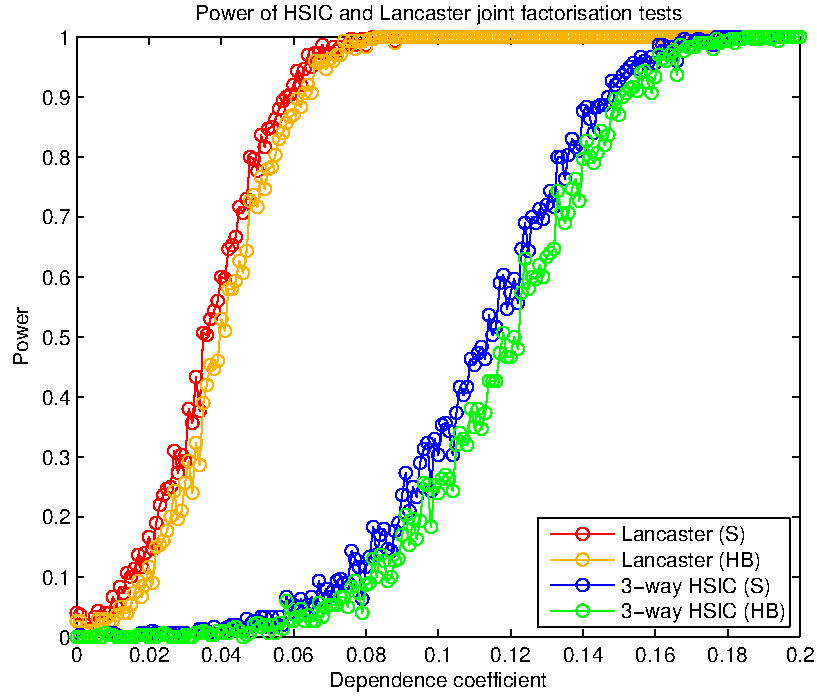
\includegraphics[scale=0.6]{UAI_Figure1.pdf}}
\caption{Results of experiment in Section \ref{experiment1}. (S) refers to the simple multiple correction; (HB) refers to Holm-Bonferroni. Observe that the Lancaster test is much more sensitive to dependence than 3-way HSIC. Note also that the test power is higher when using the simple correction when compared to the Holm-Bonferroni multiple testing correction.}
\label{weak-pairwise-strong-joint}
\end{center}
\vskip -0.2in
\end{figure} 

\subsection{False positive rates}\label{experiment2}
%Example 4 in thesis. Comparison of wild bootstrap to permutation bootstrap

This experiment demonstrates that in the time series case, existing permutation bootstrap methods fail to control the Type I error, while the  wild bootstrap correctly identifies test statistic thresholds and appropriately controls Type I error.

Synthetic data were generated from autoregressive processes $X$, $Y$ and $Z$ according to:

\begin{align*}
X_t &= aX_{t-1} + \epsilon_t\\
Y_t &= aY_{t-1} + \eta_t\\
Z_t &= aZ_{t-1} +  \zeta_t\\
\end{align*}

where $X_0, Y_0, Z_0, \epsilon_t, \eta_t$ and $\zeta_t$ are \emph{i.i.d. } $\mathcal{N}(0,1)$ random variables and $a$, called the \emph{dependence coefficient}, determines how temporally dependent the processes are. The null hypothesis in this example is true as each process is independent of the others.

The Lancaster test was performed using both the Wild Bootstrap and the simple permutation bootstrap (used in the \emph{i.i.d. } case) in order to sample from the null distributions of the test statistic. We used a fixed desired false positive rate $\alpha = 0.05$ with sample of size 1000, with 200 experiments run for each value of $a$. Figure \ref{wildBootstrap_is_necessary} shows the false positive rates for these two methods for varying $a$. It shows that as the processes become more dependent, the false positive rate for the permutation method becomes very large, and is not bounded by the fixed $\alpha$, whereas the false positive rate for the Wild Bootstrap method is bounded by $\alpha$.
\begin{figure}[ht]
\vskip 0.2in
\begin{center}
\centerline{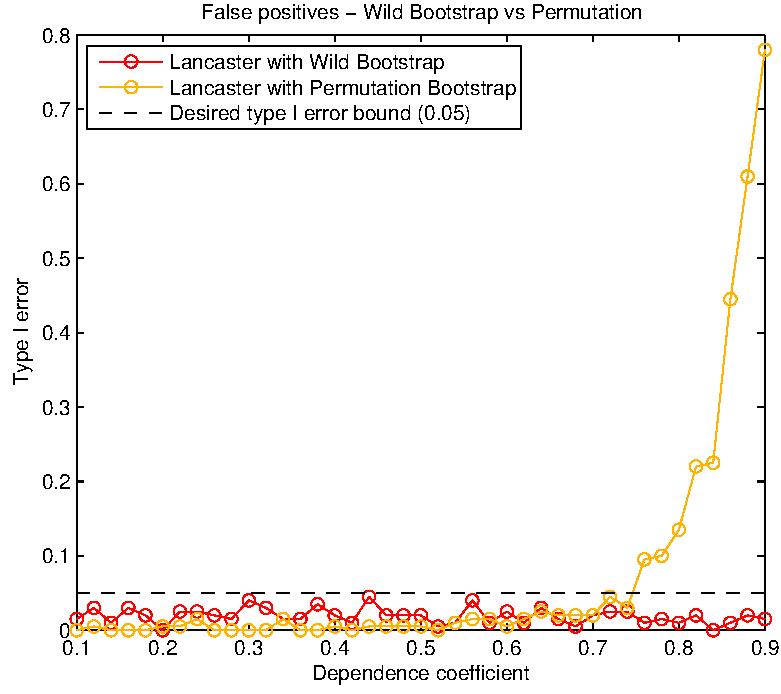
\includegraphics[scale=0.6]{UAI_Figure2.pdf}}
\caption{Results of experiment in section \ref{experiment2}. Whereas the wild bootstrap succeeds in controlling the Type I error across all values of the dependence coefficient, the permutation bootstrap fails to control the Type I error as it does not sample from the correct null distribution as temporal dependence between samples increases.}
\label{wildBootstrap_is_necessary}
\end{center}
\vskip -0.2in
\end{figure} 


\subsection{Strong pairwise interaction}\label{experiment3}
This experiment demonstrates a limitation of the Lancaster test. When pairwise interaction is strong, 3-way HSIC has greater test power than Lancaster.

Synthetic data were generated from autoregressive processes $X$, $Y$ and $Z$ according to:

\begin{align*}
X_t &= \frac{1}{2}X_{t-1} + \epsilon_t\\
Y_t &= \frac{1}{2}Y_{t-1} + \eta_t\\
Z_t &= \frac{1}{2}Z_{t-1} + d(X_t + Y_t) + \zeta_t\\
\end{align*}

where $X_0, Y_0, Z_0, \epsilon_t, \eta_t$ and $\zeta_t$ are \emph{i.i.d. } $\mathcal{N}(0,1)$ random variables and $d\in\mathbb{R}$, called the \emph{dependence} coefficient, determines the extent to which the process $(Z_t)_t$ is dependent on $X_t$ and $Y_t$.

Data were generated according to this definition with varying values for the dependence coefficient. For each value of the dependence coefficient, 300 datasets were generated, each consisting of 1200 consecutive observations of the variables. Gaussian kernels with bandwidth parameter 1 were used on each variable, and 250 bootstrapping procedures were used for each test on each dataset.

In this case $Z_t$ is pairwise-dependent on both of $X_t$ and $Y_t$, in addition to all three variables being jointly dependent. Both the Lancaster and 3-way HSIC tests should be capable of detecting the dependence and therefore reject the null hypothesis in the limit of infinite data. The results of this experiment are presented in Figure \ref{strong-pairwise}. 

Observe that in this case, the 3-way HSIC test is more sensitive to the dependence than the Lancaster test.


\begin{figure}[ht]
\vskip 0.2in
\begin{center}
\centerline{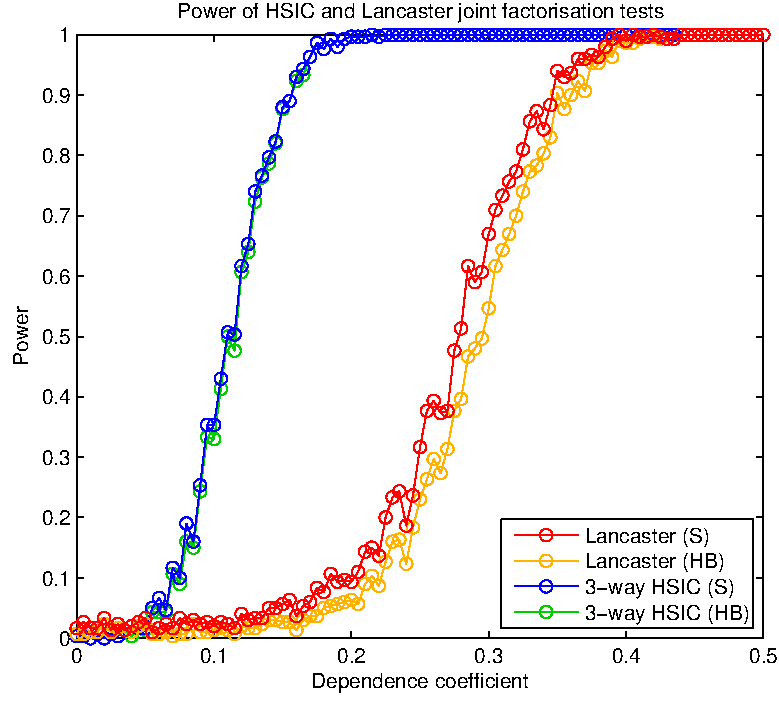
\includegraphics[scale=0.6]{UAI_Figure3.pdf}}
\caption{Results of experiment in Section \ref{experiment3}. (S) refers to the simple multiple correction; (HB) refers to Holm-Bonferroni. Observe that the Lancaster test is less sensitive to dependence than 3-way HSIC. Note also that the test power is higher when using the simple correction when compared to the Holm-Bonferroni multiple testing correction.}
\label{strong-pairwise}
\end{center}
\vskip -0.2in
\end{figure} 

\subsection{FOREX Data}

Exchange rates between three pairs of currencies (AUD/EUR, CHF/GBP, CAD/JPY) at 5 minute intervals over 7 consecutive trading days were obtained. The data were processed by taking the returns (difference between consecutive terms within each time series, $x_t^r = x_t-x_{t-1}$) which were then decomposed into volatility ($x_t^v=|x_t^r|$) and signal ($x_t^s = \mathtt{sign}(x_t^r)$) terms. The dependence of the signal and volatility terms across currency pairs were then analysed using Lancaster and 3-way HSIC, as well as (normal) HSIC to detect pairwise dependence. 

Volatility was found to be dependent across all currency pairs by each test at the $0.05$ significance level. The signals were found to be pairwise dependent by HSIC as well as jointly dependent by 3-way HSIC. Curiously, the Lancaster test did not detect dependence, with p-values of $0.682$, $0.659$ and $0.670$ for $\mathcal{H}_X$, $\mathcal{H}_Y$ and $\mathcal{H}_Z$ respectively.


\section{Discussion}

It has been demonstrated that the Lancaster test is more sensitive than 3-way HSIC when pairwise interaction is weak, but that the opposite is true when pairwise interaction is strong. It is curious that the two tests have different strengths in this manner, particularly when considering the very similar forms of the statistics in each case. Indeed, to test $\mathcal{H}_Z$ using the Lancaster statistic, we bootstrap the following:

\begin{align*}
n\|\Delta_L\hat{P}\|^2 = \frac{1}{n}\left(\widetilde{\left( \tilde{K} \circ \tilde{L}\right) }\circ \tilde{M} \right)_{++}
\end{align*}

while for the 3-way HSIC test we bootstrap:

\begin{align*}
nHSIC_b = \frac{1}{n}\left(\widetilde{\left( K \circ L\right) }\circ \tilde{M} \right)_{++}
\end{align*}

These two quantities differ only in the centring of $K$ and $L$, amounting to constant shifts in the respective feature spaces of the kernels $k$ and $l$. This difference has the consequence of quite drastically changing the types of dependency that each statistic is sensitive to.

\subsection{Directions for future research}

At present, no formal characterisation has been made of the cases in which the Lancaster statistic is more sensitive to dependence than 3-way HSIC, or why it is that modifying the feature maps of the kernels (as is implicitly done when empirically centring) should have the empirical effect on sensitivity to different types of dependence that is observed. We conjecture that other statistics could be constructed with interesting properties by choosing other ways to modify the feature maps of the kernels.

\section{Proofs}

\begin{claimproof}(Lemma \ref{lemma:hilbertCLT})

We exploit Theorem 1.1 from \cite{dehling2015bootstrap}. Using the language of this paper, $\bar{\phi}(X_i)$ is a 1-approximating functional of $(X_i)_i$, following straightforwardly from the definition of 1-approximating functionals given. 

Since our kernels are bounded, $\exists C: \enspace \|\bar{\phi}(X_i)\| < C $ and so \[\mathbb{E}\|\bar{\phi}(X_1)\|^{2+\delta} <C^{2+\delta}< \infty \enspace \forall \delta>0\]
Thus condition (1) is satisfied.

We can take $f_m = \bar{\phi}(X_0)\enspace \forall m$ and so achieve $a_m= 0 \enspace \forall m$, thus condition (2) is satisfied.

By assumption on the time series, condition (3) is satisfied.

Thus, by Theorem 1.1 in \cite{dehling2015bootstrap}
\[\sqrt{n} (\tilde{\mu}_{X} - \mu_{X}) \widesim[2]{n\longrightarrow\infty} N\]
where $N$ is a Hilbert space valued Gaussian random variable. Thus 
\[\|\tilde{\mu}_{X} - \mu_{X}\| = O(\frac{1}{\sqrt{n}})\]
\end{claimproof}


\begin{claimproof}(Theorem \ref{theorem:lancasterAsymptote})

By observing that
\begin{align*}
& \phi_X(X_i)- \frac{1}{n}\sum_k\phi_X(X_k) \\
= &  (\phi_X(X_i) - \mu_X) - \frac{1}{n}\sum_k (\phi_X(X_k) - \mu_X)\\
= &\bar\phi_X(X_i)- \frac{1}{n}\sum_k\bar\phi_X(X_k)
\end{align*}
we can therefore expand $\tilde{K}$ in terms of $\bar{K}$ as
\begin{align*}
&\tilde{K}_{ij} \\ 
&= \langle\phi_X(X_i)- \frac{1}{n}\sum_k\phi_X(X_k),\phi_X(X_j) - \frac{1}{n}\sum_k\phi_X(X_k)\rangle \\
&= \langle\bar\phi_X(X_i)- \frac{1}{n}\sum_k\bar\phi_X(X_k),\bar\phi_X(X_j) - \frac{1}{n}\sum_k\bar\phi_X(X_k)\rangle \\
&= \bar{K}_{ij} - \frac{1}{n}\sum_k\bar{K}_{ik} - \frac{1}{n}\sum_k\bar{K}_{jk} + \frac{1}{n^2}\sum_{kl}\bar{K}_{kl}
\end{align*}
and expanding $\tilde{L}$ and $\tilde{M}$ in a similar way, we can rewrite the Lancaster test statistic as

\begin{align*}
n\|\Delta_L&\hat{P}\|^2 \\&= 
\frac{1}{n}(\bar{K} \circ \bar{L}\circ \bar{M})_{++} &&-
\frac{2}{n^2}((\bar{K}\circ \bar{L}) \bar{M})_{++} \\&- 
\frac{2}{n^2}((\bar{K} \circ \bar{M}) \bar{L})_{++} &&- 
\frac{2}{n^2}((\bar{M} \circ \bar{L}) \bar{K})_{++} \\&+ 
\frac{1}{n^3}(\bar{K} \circ \bar{L})_{++} \bar{M}_{++} &&+ 
\frac{1}{n^3}(\bar{K} \circ \bar{M})_{++} \bar{L}_{++} \\&+ 
\frac{1}{n^3}(\bar{L} \circ \bar{M})_{++} \bar{K}_{++} &&+ 
\frac{2}{n^3}(\bar{M}\bar{K}\bar{L})_{++} \\&+ 
\frac{2}{n^3}(\bar{K}\bar{L}\bar{M})_{++} &&+ 
\frac{2}{n^3}(\bar{K}\bar{M}\bar{L})_{++} \\&+ 
\frac{4}{n^3}tr(\bar{K}_+ \circ \bar{L}_+ \circ \bar{M}_+) &&-
\frac{4}{n^4}(\bar{K} \bar{L})_{++} \bar{M}_{++} \\& - 
\frac{4}{n^4}(\bar{K}\bar{M})_{++}\bar{L}_{++} &&- 
\frac{4}{n^4}(\bar{L}\bar{M})_{++} \bar{K}_{++} \\&+
\frac{4}{n^5}\bar{K}_{++} \bar{L}_{++} \bar{M}_{++} \\
\end{align*}

Each of these terms can be expressed as inner products between empirical estimates of population centred covariance operators and tensor products of mean embeddings. Rewriting them as such yields:
\begin{align*}
n\|\Delta_L \hat{P}\|^2 &= n\langle \bar{C}_{XYZ},\bar{C}_{XYZ} \rangle \\& -
2n\langle \bar{C}_{XYZ},\bar{C}_{XY}\otimes\bar{\mu}_Z \rangle \\& -
2n\langle \bar{C}_{XZY},\bar{C}_{XZ}\otimes\bar{\mu}_Y \rangle \\& -
2n\langle \bar{C}_{YZX},\bar{C}_{YZ}\otimes\bar{\mu}_X \rangle \\& +
n\langle \bar{C}_{XY}\otimes\bar{\mu}_Z,\bar{C}_{XY}\otimes\bar{\mu}_Z \rangle \\& +
n\langle \bar{C}_{XZ}\otimes\bar{\mu}_Y,\bar{C}_{XZ}\otimes\bar{\mu}_Y \rangle \\& +
n\langle \bar{C}_{YZ}\otimes\bar{\mu}_X,\bar{C}_{YZ}\otimes\bar{\mu}_X \rangle \\& +
2n\langle \bar{\mu}_Z\otimes\bar{C}_{XY},\bar{C}_{ZX}\otimes\bar{\mu}_Y \rangle \\& +
2n\langle \bar{\mu}_X\otimes\bar{C}_{YZ},\bar{C}_{XY}\otimes\bar{\mu}_Z \rangle \\& +
2n\langle \bar{\mu}_X\otimes\bar{C}_{ZY},\bar{C}_{XZ}\otimes\bar{\mu}_Y \rangle \\& +
4n\langle \bar{C}_{XYZ},\bar{\mu}_X \otimes\bar{\mu}_Y \otimes \bar{\mu}_Z \rangle \\& -
4n\langle \bar{C}_{XY}\otimes \bar{\mu}_Z,\bar{\mu}_X \otimes\bar{\mu}_Y \otimes \bar{\mu}_Z \rangle \\& -
4n\langle \bar{C}_{XZ}\otimes \bar{\mu}_Y,\bar{\mu}_X \otimes\bar{\mu}_Z \otimes \bar{\mu}_Y \rangle \\& -
4n\langle \bar{C}_{YZ}\otimes \bar{\mu}_X,\bar{\mu}_Y \otimes\bar{\mu}_Z \otimes \bar{\mu}_X \rangle \\& +
4n\langle \bar{\mu}_X \otimes\bar{\mu}_Y \otimes \bar{\mu}_Z,\bar{\mu}_X \otimes\bar{\mu}_Y \otimes \bar{\mu}_Z \rangle \\
\end{align*}
By assumption, $\mathbb{P}_{XYZ} =\mathbb{P}_{XY}\mathbb{P}_{Z}$ and thus the expectation operator also factorises similarly. As a consequence, 
\begin{align*}
C_{XYZ} &= \mathbb{E}_{XYZ}[\bar\phi_X(X)\otimes\bar\phi_Y(Y)\otimes\bar\phi_Z(Z)] \\
& = \mathbb{E}_{XY}[\bar\phi_X(X)\otimes\bar\phi_Y(Y)]\otimes\mathbb{E}_{Z}\bar\phi_Z(Z)=0
\end{align*}

Similarly, $C_{XZY}$, $C_{YZX}$, $C_{XZ}$, $C_{YZ}$ are all 0 in their respective Hilbert spaces. Lemma \ref{lemma:beta} tells us that each subprocess of $(X_i,Y_i,Z_i)$ satisfies the same $\beta$-mixing conditions as $(X_i,Y_i,Z_i)$, thus by applying Lemma \ref{lemma:hilbertCLT} it follows that $\|\bar{C}_{XZY}\|$, $\|\bar{C}_{YZX}\|$, $\|\bar{C}_{XZ}\|$, $\|\bar{C}_{YZ}\|$, $\|\bar{\mu}_X\|$, $\|\bar{\mu}_Y\|$, $\|\bar{\mu}_Z\| = O\left(\frac{1}{\sqrt{n}}\right)$

It thus follows that
\begin{align*}
n\|\Delta_L& \hat{P}\|^2  \xrightarrow{O(n^{-\frac{1}{2}})} n\langle \bar{C}_{XYZ},\bar{C}_{XYZ} \rangle \\ &-
2n\langle \bar{C}_{XYZ},\bar{C}_{XY}\otimes\bar{\mu}_Z \rangle -
2n\langle \bar{C}_{XZY},\bar{C}_{XZ}\otimes\bar{\mu}_Y \rangle \\ &=
\frac{1}{n}((\bar{K}\circ \bar{L}) \circ \bar{M})_{++}\\& - \frac{2}{n^2}((\bar{K}\circ \bar{L})\bar{M})_{++} + \frac{1}{n^3}(\bar{K}\circ \bar{L})_{++}\bar{M}_{++}
\end{align*}

since all the other terms decay at least as quickly as $O(\frac{1}{\sqrt{n}})$. This is shown here for $n\langle \bar{\mu}_X\otimes\bar{C}_{YZ},\bar{C}_{XY}\otimes\bar{\mu}_Z \rangle$; the proofs for the other terms are similar.
\begin{align*}
&n\langle \bar{\mu}_X\otimes\bar{C}_{YZ},\bar{C}_{XY}\otimes\bar{\mu}_Z \rangle \\
&\leq n \| \bar{\mu}_X\otimes\bar{C}_{YZ}\| \|\bar{C}_{XY}\otimes\bar{\mu}_Z \| \\
& = n\sqrt{\langle \bar{\mu}_X\otimes\bar{C}_{YZ} , \bar{\mu}_X\otimes\bar{C}_{YZ} \rangle} \sqrt{\langle \bar{C}_{XY}\otimes\bar{\mu}_Z, \bar{C}_{XY}\otimes\bar{\mu}_Z \rangle} \\
& = n\sqrt{\langle \bar{\mu}_X, \bar{\mu}_X \rangle \langle \bar{C}_{YZ} , \bar{C}_{YZ} \rangle} \sqrt{\langle \bar{C}_{XY}, \bar{C}_{XY} \rangle \langle \bar{\mu}_Z, \bar{\mu}_Z \rangle} \\
& =  n \| \bar{\mu}_X\|\|\bar{C}_{YZ}\| \|\bar{C}_{XY}\|\|\bar{\mu}_Z \| \\
& = n \mathsmaller{O\left(\frac{1}{\sqrt{n}}\right)} \mathsmaller{O\left(\frac{1}{\sqrt{n}}\right)} O(1) \mathsmaller{O\left(\frac{1}{\sqrt{n}}\right)} = \mathsmaller{O\left(\frac{1}{\sqrt{n}}\right)}
\end{align*}

It can be shown that $\bar{K}\circ \bar{L}$ in the above expression can be replaced with $\overline{\bar{K}\circ \bar{L}}$ while preserving equality. That is, we can equivalently write
\begin{align*}
n\|\Delta_L \hat{P}\|^2 & \longrightarrow \frac{1}{n}((\overline{\bar{K}\circ \bar{L}}) \circ \bar{M})_{++}\\& - \frac{2}{n^2}((\overline{\bar{K}\circ \bar{L}})\bar{M})_{++} + \frac{1}{n^3}(\overline{\bar{K}\circ \bar{L}})_{++}\bar{M}_{++}
\end{align*}
This is equivalent to treating $\bar{k}\otimes\bar{l}$ as a kernel on the single variable $T:=(X,Y)$ and performing another recentering trick as we did at the beginning of this proof. By rewriting the above expression in terms of the operator $\bar{C}_{TZ}$ and mean embeddings $\mu_T$ and $\mu_Z$, it can be shown by a similar argument to before that the latter two terms tend to 0 at least as $O(\frac{1}{n})$, and thus  
\begin{align*}
n\|\Delta_L \hat{P}\|^2 \xrightarrow{O(\frac{1}{\sqrt{n}})} \frac{1}{n}((\overline{\bar{K}\circ \bar{L}}) \circ \bar{M})_{++}
\end{align*} as required.

To show that this is a normalised degenerate V-statistic observe that, writing $S_i=(X_i,Y_i,Z_i)$ and $h(S_i,S_j) = \langle\bar{\phi}(X_i)\otimes\bar{\phi}(Y_i) - C_{XY},\bar{\phi}(X_j)\otimes\bar{\phi}(Y_j) - C_{XY}\rangle\langle\bar{\phi}(Z_i),\bar{\phi}(Z_j)\rangle$, we can write:
\begin{align*}
&\frac{1}{n}((\overline{\bar{K}\circ \bar{L}}) \circ \bar{M})_{++}= \frac{1}{n}\sum_{ij} h(S_i,S_j)
\end{align*}

And thus it is a normalised V-statistic. To show that it is degenerate, fix any $s_i$ and observe that $\mathbb{E}_{S_j}h(s_i,S_j)=0$ since $\mathbb{E}_{XYZ} =\mathbb{E}_{XY}\mathbb{E}_{Z}$.

\end{claimproof}



\section*{Acknowledgments} 
Big up to all my homies

\subsubsection*{References}
\bibliography{ref}



%%%%%%%%%%%%%%%%%%%%%%%%%%%%%%%%%%%%%%%%%%%
%%%%%%%%%%%%%%%%%%%%%%%%%%%%%%%%%%%%%%%%%%%
\appendix
\onecolumn

\section{Supplementary material}
This supplementary section contains a proof of Lemma \ref{lemma:beta} and a proof that the HSIC statistic asymptotically satisfies the hypothesis of the Wild Bootstrap.

\subsection{Proof of Lemma \ref{lemma:beta}}

\begin{claimproof}(Lemma \ref{lemma:beta}) 

Let us consider $(X_t,Y_t)_t$.
Let us call $\beta_{XYZ}(m)$ the coefficients for the process $(X_t,Y_t,Z_t)_t$, and $\beta_{XY}(m)$ the coefficients for the process $(X_t,Y_t)_t$. 

Observe that for $A \in \sigma((X_b,Y_b),\ldots, (X_c,Y_c))$, it is the case that $A \times \mathcal{Z} \in \sigma((X_b,Y_b,Z_b),\ldots, (X_c,Y_c,Z_c))$ and $\mathbb{P}_{XY}(A) = \mathbb{P}_{XYZ}(A\times \mathcal{Z})$.

Thus

\begin{align*}
\beta_{XY}(m) &= \frac{1}{2} \sup_n \sup_{ \{A_i^{XY} \}, \{B_j^{XY} \} } \sum_{i=1}^I \sum_{j=1}^J | \mathbb{P}_{XY}(A_i^{XY} \cap B_j^{XY}) - \mathbb{P}_{XYZ}(A_i^{XY})\mathbb{P}_{XYZ}(B_j^{XY})| \\
&= \frac{1}{2} \sup_n \sup_{ \{A_i^{XY} \}, \{B_j^{XY} \} } \sum_{i=1}^I \sum_{j=1}^J | \mathbb{P}_{XYZ}((A_i^{XY}\times \mathcal{Z}) \cap (B_j^{XY} \times \mathcal{Z})) \\& \quad \quad\quad \quad \quad \quad\quad \quad \quad \quad\quad \quad- \mathbb{P}_{XYZ}(A_i^{XY}\times \mathcal{Z})\mathbb{P}_{XYZ}(B_j^{XY} \times \mathcal{Z})| \\
& \leq \frac{1}{2} \sup_n \sup_{ \{A_i^{XYZ} \}, \{B_j^{XYZ} \} } \sum_{i=1}^I \sum_{j=1}^J | \mathbb{P}_{XYZ}(A_i^{XYZ} \cap B_j^{XYZ}) - \mathbb{P}_{XYZ}(A_i^{XYZ})\mathbb{P}_{XYZ}(B_j^{XYZ})| \\
& = \beta_{XYZ}(m)
\end{align*}

Thus we have shown that  $\beta_{XYZ}(m) \longrightarrow 0 \implies \beta_{XY}(m) \longrightarrow 0$. That is, if  $(X_t,Y_t,Z_t)_t$ is $\beta$-mixing then so is  $(X_t,Y_t)_t$ 

A similar argument holds for any other sub-process.
\end{claimproof}

\subsection{Proof that HSIC can be Wild Bootstrapped}

Given samples $\{(X_i,Y_i)\}_{i=1}^n$, and taking all notation involving kernels and base spaces as before, the HSIC statistic is defined to be the squared RKHS distance between the empirical embeddings of the distributions $\mathbb{P}_{XY}$ and $\mathbb{P}_X\mathbb{P}_Y$:

\begin{align*}
HSIC_b & = \| \frac{1}{n}\sum_i \phi_X(X_i) \otimes \phi_Y(Y_i) - \left(\frac{1}{n}\sum_i \phi_X(X_i)\right) \otimes \left(\frac{1}{n}\sum_i \phi_Y(Y_i) \right)\|^2 \\
& = \frac{1}{n^2} (K\circ L)_{++}  - \frac{2}{n^3}(KL)_{++} + \frac{1}{n^4}K_{++}L_{++} \\
& = \frac{1}{n^2}(\tilde{K}\circ \tilde{L})_{++}
\end{align*}
where the last equality can be shown easily by expanding $\tilde{K}$ (and $\tilde{L}$ similarly) as
\begin{align*}
\tilde{K}_{ij} &= \langle\phi_X(X_i)- \frac{1}{n}\sum_k\phi_X(X_k),\phi_X(X_j) - \frac{1}{n}\sum_k\phi_X(X_k)\rangle \\
&= K_{ij} - \frac{1}{n}\sum_kK_{ik} - \frac{1}{n}\sum_kK_{jk} + \frac{1}{n^2}\sum_{kl}K_{kl}
\end{align*} 

\begin{theorem}
Suppose that $\mathbb{P}_{XY} = \mathbb{P}_X\mathbb{P}_Y$. Then 
\begin{align*}
nHSIC_b & \xrightarrow{O(n^{-\frac{1}{2}})} \frac{1}{n} (\bar{K}\circ \bar{L})_{++}
\end{align*}
and this is a normalised degenerate V-statistic.
\end{theorem}

\begin{proof}
By writing
\begin{align*}
\tilde{K}_{ij} &= \bar{K}_{ij} - \frac{1}{n}\sum_k\bar{K}_{ik} - \frac{1}{n}\sum_k\bar{K}_{jk} + \frac{1}{n^2}\sum_{kl}\bar{K}_{kl}
\end{align*} 
and similar for $\tilde{L}$ we can rewrite $nHSIC_b$ as 
\begin{align*}
nHSIC_b & = \frac{1}{n} (\bar{K}\circ \bar{L})_{++}  - \frac{2}{n^2}(\bar{K}\bar{L})_{++} + \frac{1}{n^3}\bar{K}_{++}\bar{L}_{++} \\
\end{align*}
We will show that the latter two terms in the above expression decay to 0 as $n\longrightarrow\infty$. 

By assumption, $\mathbb{P}_{XY} = \mathbb{P}_X\mathbb{P}_Y$ and thus the expectation operator factorises similarly. Therefore 
\begin{align*}
C_{XY} & = \mathbb{E}_{XY}[\bar{\phi}_X(X)\otimes\bar{\phi}_Y(Y)] \\
& = \mathbb{E}_{X}[\bar{\phi}_X(X)]\otimes\mathbb{E}_Y[\bar{\phi}_Y(Y)] = 0\otimes 0 = 0\\
\end{align*}

Thus by Lemma \ref{lemma:hilbertCLT} as before, it follows that $\|\bar{C}_{XY}\|, \|\bar{\mu}_X\|, \|\bar{\mu}_Y\| = O(n^{-\frac{1}{2}})$. 

We can write the latter two terms in the above expression for $nHSIC_b$ in terms of these quantities:

\begin{align*}
\frac{1}{n^2}(\bar{K}\bar{L})_{++} &= \frac{1}{n^2} \sum_{ijk}\bar{K}_{ij}\bar{L}_{jk}\\
&= \frac{1}{n^2} \sum_{ijk}\langle \bar{\phi}_X(X_i),\bar{\phi}_X(X_j) \rangle \langle \bar{\phi}_Y(Y_j),\bar{\phi}_Y(Y_k)\rangle \\&=
\frac{1}{n^2} \sum_{ijk}\langle \bar{\phi}_X(X_j)\otimes\bar{\phi}_Y(Y_j),
\bar{\phi}_X(X_i)\otimes\bar{\phi}_Y(Y_k)\rangle \\&=
n\langle \frac{1}{n} \sum_{j}[\bar{\phi}_X(X_j)\otimes\bar{\phi}_Y(Y_j)],
[\frac{1}{n} \sum_{i}\bar{\phi}_X(X_i)]\otimes[\frac{1}{n} \sum_{k}\bar{\phi}_Y(Y_k)]\rangle \\&=
n\langle \bar{C}_{XY},\bar{\mu}_X  \otimes \bar{\mu}_Y \rangle \\ 
&\leq n \|\bar{C}_{XY}\|\|\bar{\mu}_X\| \| \bar{\mu}_Y\|\\
&= O(n^{-\frac{1}{2}})
\end{align*}

\begin{align*}
 \frac{1}{n^3}\bar{K}_{++}\bar{L}_{++} &= \frac{1}{n^3}\mathlarger{\mathlarger{\sum}}_{i,j}\bar{K}_{ij}\bar{L}_{ij}\\
 & =  \frac{1}{n^3}\mathlarger{\mathlarger{\sum}}_{i,j}\mathlarger{\mathlarger{\langle}} \bar{\phi}_X(X_i), \bar{\phi}_X(X_j) \mathlarger{\mathlarger{\rangle}} \mathlarger{\mathlarger{\sum}}_{k,l}\mathlarger{\mathlarger{\langle}} \bar{\phi}_Y(Y_k), \bar{\phi}_Y(Y_l) \mathlarger{\mathlarger{\rangle}} \\ &
 = n\mathlarger{\mathlarger{\langle}} \frac{1}{n}\sum_i\bar{\phi}_X(X_i) , \frac{1}{n}\sum_j\bar{\phi}_X(X_j) \mathlarger{\mathlarger{\rangle}} \mathlarger{\mathlarger{\langle}} \frac{1}{n}\sum_k\bar{\phi}_Y(Y_k)  , \frac{1}{n}\sum_l\bar{\phi}_Y(Y_l) \mathlarger{\mathlarger{\rangle}}\\&
 = n \mathlarger{\mathlarger{\langle}} \bar{\mu}_X , \bar{\mu}_X \mathlarger{\mathlarger{\rangle}} \mathlarger{\mathlarger{\langle}} \bar{\mu}_Y , \bar{\mu}_Y  \mathlarger{\mathlarger{\rangle}} \\ &
= n\|\bar{\mu}_X \|^2 \|\bar{\mu}_Y \|^2\\ &= nO(n^{-2}) \\&= O(n^{-1})
\end{align*}


It follows that $nHSIC_b  \xrightarrow{O(n^{-\frac{1}{2}})} \frac{1}{n} (\bar{K}\circ \bar{L})_{++}$

To show that this is a normalised degenerate V-statistic observe that, writing $S_i=(X_i,Y_i)$ and $h(S_i,S_j) = \langle\bar{\phi}(X_i),\bar{\phi}(X_j)\rangle \langle\bar{\phi}(Y_i),\bar{\phi}(Y_j)\rangle$, we can write:
\begin{align*}
 \frac{1}{n} (\bar{K}\circ \bar{L})_{++}= \frac{1}{n}\sum_{ij} h(S_i,S_j)
\end{align*}

and thus it is a normalised V-statistic. To show that it is degenerate, fix any $s_i$ and observe that 
\begin{align*}
\mathbb{E}_{S}h(s_i,S) &= \mathbb{E}_X\mathbb{E}_Y \langle\bar{\phi}(x_i),\bar{\phi}(X)\rangle \langle\bar{\phi}(y_i),\bar{\phi}(Y)\rangle \\
&= \langle\bar{\phi}(x_i),\mathbb{E}_X\bar{\phi}(X)\rangle \langle\bar{\phi}(y_i),\mathbb{E}_Y\bar{\phi}(Y)\rangle \\
&= \langle\bar{\phi}(x_i),0\rangle \langle\bar{\phi}(y_i),0\rangle = 0\\
\end{align*}	
\end{proof}

\end{document}
